%%%%%%%%Bilecik �eyh Edebali �niversitesi M�hendsilik Fak�ltesi%%%%
%%%%%%%%%%%Bilgisayar M�hendisli�i Proje I-II �al��mas�%%%%%%%%%%%%
%%%%%%%%%%%%%%%%%%%%%%LaTeX Class%%%%%%%%%%%%%%%%%%%%%%%%%%%%%%%%%%
\documentclass{BUP}
\usepackage[numbered,framed]{matlab-prettifier}
\usepackage{listings}

%\lstloadlanguages{C,C++,csh,java,php}
%\ltsloadlanguages{Matlab}
%%%%%%%%%%%%%%%%%%%%%%%%%%%%%%%%%%%%%%%%%%%%%%%%%%%%%%%%%%%%%%%%%%%%%%%%%%%
\begin{document}
\shorthandoff{=}%grafik komutlar�nda babelden kaynaklanan hatay� engeller.
%%%%%%%%%%%%%Proje I-II �al��malar�n�n B�l�mleri%%%%%%%%%%%%%%%%%%%%%%%%%%%
\thispagestyle{empty} %Bu sayfaya sayfa numaralar� yaz�lmaz
\begin{figure}[H]
\centering

\includegraphics[scale=0.2]{logomuz}
%Bu komutla resim dosyam�z� y�kl�yoruz.
\end{figure}
%sa�a 4 sol 2 a�a�� yukar� 3%
\begin{center}
\textbf{T.C.}\\
\textbf{B�LEC�K �EYH EDEBAL� �N�VERS�TES�}\\
\textbf{M�HEND�SL�K FAK�LTES�}

\textbf{B�LG�SAYAR M�HEND�SL��� B�L�M�}
\end{center}

\vspace*{4cm}%bir miktar bo�luk b�rakmak i�in
\begin{center}
\textbf{MATLAB UYGULAMALARININ WEB API �LE �ALI�TIRILMASI}

\textbf{Zeynep KOTAN}

\textbf{Bilgisayar M�hendisli�i Tasar�m �al��mas� II}
\end{center}

\vspace*{\fill}
\begin{center}
\textbf{PROJE II DANI�MANI : ��r. G�r. Yusuf MU�TU }

\textbf{B�LEC�K}\\ 
\textbf{\today}
\end{center}

\thispagestyle{empty} %Bu sayfaya sayfa numaralar� yaz�lmaz

\begin{figure}[H]
\centering

\includegraphics[scale=0.2]{logomuz}
%Bu komutla resim dosyam�z� y�kl�yoruz.
\end{figure}
%sa� 4 sol 2 a�a�� yukar� 3%
\begin{center}
\textbf{T.C.}\\
\textbf{B�LEC�K �EYH EDEBAL� �N�VERS�TES�}\\
\textbf{M�HEND�SL�K FAK�LTES�}

\textbf{B�LG�SAYAR M�HEND�SL��� B�L�M�}
\end{center}

\vspace*{4cm}%bir miktar bo�luk b�rakmak i�in
\begin{center}
\textbf{
MATLAB UYGULAMALARININ WEB API �LE �ALI�TIRILMASI}

\textbf{Zeynep KOTAN}

\textbf{Bilgisayar M�hendisli�i Tasar�m �al��mas� II}
\end{center}

\vspace*{\fill}
\begin{center}
\textbf{PROJE II DANI�MANI : ��r. G�r. Yusuf MU�TU}

\textbf{B�LEC�K}\\ 
\textbf{\today}
\end{center}

\pagenumbering{roman}%romen rakamlar� kullan�lmaya ba�lan�yor.
\setcounter{page}{2}% sayfa numaras�n� ii'den ba�lat�l�yor.
\centerline{\bf �ZET}
\addcontentsline{toc}{section}{�ZET}

\begin{center}
\textbf{Projenin Amac�}
\end{center}
\qquad Bu proje sayesinde  m�hendislik ve teknik e�itimde s�k�a kullan�lan MATLAB uygulamas�n�n Web tabanl� olarak ger�ekle�tirilmesi hedeflenmi�tir. Web sayfas�nda File Upload i�lemi yaparak se�ti�imiz resim Matlab'a g�nderilir.  G�r�nt� i�leme ile resimdeki ki�i say�s� bulunur. Ard�ndan ki�i say�s�  Web'de yazd�r�l�r. 
\begin{center}
\textbf{Projenin Kapsam�}
\end{center}
\qquad Matlab uygulamas� olarak g�n�m�z de yayg�n olan g�r�nt� i�leme esas al�nm��t�r. G�r�nt� ��lemenin �ok �e�itli ve farkl� uygulamalar� olmakla birlikte g�r�nt� i�leme, pek �ok alanda kullan�lmaktad�r. S�z konusu yo�un kullan�m alanlar�n�n internet �zerinde icra edilmesi ile g�r�nt� i�leme kapsam�nda web tabanl� �e�itli proje, �al��ma ve ara�t�rma gibi uygulamalar ger�ekle�tirilebilir. Ayr�ca aray�z�n web tabanl� tasarlanmas�yla, y�ntemin yayg�nla�t�r�lmas�, zaman kayb�n� ortadan kald�rarak birden fazla kullan�c�n�n e� zamanl� kullanabilmesi ama�lanm��t�r.


%%%%%%%%%%%%%%%%%%%%%%%%%%%%%%%%%%%%%%%ABSTRACT%%%%%%%%%%%%%%%%%%%%%%%%%%%%%%%%%%%%%%%%%%
\newpage
\centerline{\bf ABSTRACT}
\addcontentsline{toc}{section}{ABSTRACT}
\begin{center}
\textbf{Project Objective}
\end{center}

 Thanks to this project has been targeted frequently used in education of engineering and technical realization as a Web-based MATLAB applications. File Web page 
choose Upload making process images sent to MATLAB. The number of people located in the picture with the image processing. Then the number of people is printed on the web[5].


%Bilecik �eyh Edebali University Department of Computer Engineering students is studied. The aim of project is work to create a template for writing \LaTeX\ writing the final report template in the Project, to be written.

\begin{center}
\textbf{Scope of Project}
\end{center}
\qquad Today as Matlab image processing applications have also been widespread basis. While a variety of different image processing and image processing applications, however, are used in many fields. Said intensive use of the area covered by the image processing to be carried out on the internet with various web-based projects, such as studies and research carried out applications. In addition, by designing the web-based interface, dissemination methods, eliminating the time-consuming aimed multiple users can use simultaneously[5].


%Bilecik �eyh Edebali University Computer Engineering Department Bilecik need to create a project template Latex codes assignment, involves the use of. The first part of the project consists of two parts, \LaTeX's development have been studied and why it is preferred that the use of information provided in the information. Faculty of Engineering of the university for the second part, Sheikh Edebali Bilecik Project Paper \LaTeX\ codes and are included.


\addcontentsline{toc}{section}{TE�EKK�R}
\section*{TE�EKK�R}
Bu projenin ba��ndan sonuna kadar haz�rlanmas�nda  eme�i bulunan ve 
beni bu konuya y�nlendiren sayg�de�er hocam ve dan��man�m 
Say�n ��r. G�r. Yusuf MU�TU'ya t�m katk�lar�ndan ve hi� 
eksiltmedi�i deste�inden dolay� te�ekk�r ederim.
\vspace{2cm}

\begin{flushright}
\textbf{Zeynep KOTAN}

\today
\end{flushright}
\tableofcontents%bu komutun oldu�u yerde i�indekiler olu�turulur.
%\textbf{\centerline{\bf S�MGE L�STES�}}
\addcontentsline{toc}{section}{S�MGE L�STES�}

\renewcommand*\listfigurename{\centerline{\bf\normalsize �EK�L L�STES�}}
\listoffigures%bu komutun oldu�u yerde �ekiller listesi olu�turulur
\addcontentsline{toc}{section}{�EK�L L�STES�}
%\renewcommand*\listtablename{\centerline{\bf\normalsize TABLO L�STES�}}
\listoftables%bu komutun oldu�u yerde tablolar listesi olu�turulur
\addcontentsline{toc}{section}{TABLO L�STES�}
\pagenumbering{arabic}%Sayfa numaralamas�n� arap rakamlar�yla yapar.
\setcounter{page}{1}%sayfa numaras�n� 1'den ba�lat�r.
\section{G�R��}
\qquad G�n�m�zde bilgisayarlar ya�ant�m�z�n vazge�ilmez bir par�as� haline gelmi�tir. Akla gelebilecek her alanda bilgisayar�n kullan�m� g�r�lmektedir. �zellikle bu �al��mada yap�lan uygulama g�z �n�ne al�nd���nda bilgisayar destekli e�itim, ara�t�rma, g�r�nt� i�leme ve benzetim uygulamalar� a��s�ndan bilgisayarlar�n kullan�c�lara �ok b�y�k oranda kolayl�k sa�lad��� a��k bi�imde g�r�lmektedir. Bilgisayar kullan�m�n�n getirdi�i kolayl�klar yan�nda daha bir�ok avantajlar� bulunmaktad�r. Bu avantajlardan baz�lar� bilgisayar destekli analiz ve benzetim aray�zleri temelinde s�ralan�rsa;
\begin{itemize}
\item Denenmesi riskli ve tehlikeli olan olaylar�n deneysel �al��maya ihtiya� duyulmadan incelenmesi sa�lan�r,
\item ��lemlerin otomatik olarak bilgisayar ortam�nda ger�ekle�tiriliyor olmas� zaman ve maliyetten tasarruf edilmesini ve en az hata ile daha verimli bir �al��ma yap�lmas�n� sa�lar,
\item Kullan�c� say�s�nda s�n�rlama olmaks�z�n i�lemlerin defalarca tekrarlanmas�na olanak sa�lar, 
\item Elde edilen say�sal veriler kolayl�kla grafik haline d�n��t�r�lebilir,
\item Yap�lan i�lemler hakk�nda g�rsel bir de�erlendirme ve kar��la�t�rma yap�labilir.
\end{itemize}
\qquad S�ralanan t�m bu avantajlar sayesinde bilgisayarlar ile ger�ekle�tirilen benzetim ve analiz uygulamalar� bilgisayar destekli e�itim, uzaktan e�itim, ara�t�rma-geli�tirme alanlar�nda olduk�a yayg�n bi�imde kullan�lmaktad�r. Bu ama�la yap�lm�� aray�z temelli �al��malarda birka� farkl� platformdan yararlan�labilir. �rne�in MATLAB GUI ile haz�rlanan bu aray�zler MATLAB'�n geli�mi� analiz ve grafik �zelliklerini kulland�klar�nda �ok esnek ve kullan��l� bir yap�ya sahiptirler. Ancak bu platformda haz�rlanan aray�zlerin �al��mas� i�in o bilgisayarda MATLAB program�n�n y�kl� olmas� gerekmektedir. MATLAB'a olan bu ba��ml�l�k hem maliyet hem de haz�rlanan aray�z�n ta��nabilirli�i a��s�ndan dezavantaj olu�turmaktad�r. MATLAB GUI i�in ortaya konan dezavantajlar�n giderilmesi i�in daha genel kullan�ma y�nelik platformlar (Flash, .NET gibi) ile aray�zler haz�rlanabilir. Bu �ekilde yap�lan bir uygulama herhangi bir bilgisayarda farkl� bir yaz�l�ma ihtiya� duymaks�z�n �al��t�r�labilir bir yap�ya sahip oldu�undan hem maliyet hem de ta��nabilirlik a��s�ndan avantaj sa�lar. Ayr�ca .NET platformu C\#, ASP.NET, VB.NET gibi diller i�in ortak bir platform oldu�undan uygulaman�n geli�tirilmesi s�ras�nda bu dillerden birlikte yararlan�labilme imkan� vard�r.

\qquad Aray�z tasar�m�nda kullan�labilecek ���nc� yakla��m ise MATLAB ve .NET platformlar�n�n avantajlar�na sahip olan bir yap�d�r. Hatta bu yakla��m ile bu avantajlar� bir ad�m daha �teye ta��yarak web temelli yap�ya kavu�turmak ve yap�lan uygulaman�n yayg�nla�mas�n� sa�lamak da m�mk�nd�r.

\qquad Son y�llarda �zellikle m�hendislik e�itimine y�nelik internet tabanl� e�itimsel aray�z �al��malar� h�z kazanm��t�r. Konuyla ilgili literat�rde �ok say�da �al��ma mevcuttur. Bu �al��malar incelendi�inde MATLAB program�n�n ger�ekle�tirilen uygulamalarda temel ara�lardan bir tanesi oldu�u g�r�lmektedir. MATLAB program�n�n �zelliklerini web temelli uygulamalara aktarmak i�in g�n�m�zde MATLAB Builder NE ve MATLAB Web Figure ara�lar� kullan�lmaktad�r. Bu ara�lar ile MATLAB'ta haz�rlanan fonksiyonlar .NET bile�enlerine d�n��t�r�lerek kullan�lmaktad�r. Bu yakla��ma �rnek olarak haz�rlam�� oldu�um ki�i say�s� analizini verilebilinir.

\section{MATERYAL VE METODLAR}
\qquad Bu b�l�mde kullan�lan materyal ve metodlardan bahsedilecektir. Projede kullan�lan materyaller:
\begin{itemize}
\item MATLAB
\item VISUAL STUDIO
\item POSTMAN
\end{itemize}

\qquad Se�ilen materyallerin neden se�ildigi hakk�nda k�saca bilgilendireyim. Matlab  G�r�nt� ��leme alan�nda uygulama geli�tirmek i�in gereklidir. Visual Studio ise File upload i�lemini yaparak Matlab da olu�turdu�umuz dll'e resmi g�ndererek sonucu yazd�rma i�lemini yap�yor. Postman ise Visual Studio'da yaz�lan Api'yi test etmek, payla�mak, dok�mante ve monit�r elde etmek i�in kullan�lan aray�zd�r.
\subsection{MATLAB}

\qquad MATLAB, genellikle pozitif bilim ve m�hendislik hesaplamalar� i�in kullan�lan bir bilgisayar program�d�r. Amerika Birle�ik Devletleri merkezli MathWorks firmas� taraf�ndan geli�tirilen MATLAB, ayn� zamanda bir programlama dilidir. �ngilizce "Matrix Laboratory" kelimelerinin birle�tirilmesi ile olu�mu� olan MATLAB, isminden de anla��laca�� gibi matris tabanl� bir �al��ma sistemine sahiptir.
Lineer cebir, istatistik, optimizasyon, n�merik analiz, optimizasyon, fourier analizi gibi pek �ok matematiksel hesaplaman�n etkili ve h�zl� �ekilde yap�lmas�na olanak sa�layan MATLAB program� ayn� zamanda 2D ve 3D grafik �izimi i�in de kullan�l�r.

\qquad MATLAB ile kullan�c�lar kendi programlar�n� haz�rlayabilirler. Matrisler ve onlar�n etkile�im i�inde oldu�u fonksiyonlarla programlama yap�lmas�na izin veren MATLAB ile �ok karma��k matematik hesaplamalar� bile birka� saniye i�inde tamamlan�r. Temel programlama fonksiyonlar� ile benzer fonksiyonlar�n kullan�labildi�i MATLAB ile etkili ve pratik programlar haz�rlanabilir.

\qquad C, Java gibi programlama dillerindeki dizilerin kullan�m� ile ayn� mant�kla matrislerin kullan�ld��� MATLAB program�nda bir, iki veya daha fazla boyutta matrisler ile �al��mak m�mk�nd�r.
MATLAB ile temel matematik fonksiyonlar�n�n iki ve �� boyutlu grafikleri �izilebilir. Polinomlar, parboller, sin�s dalgalar� ba�ta olmak �zere her t�r iki ve �� boyutlu matematiksel grafik MATLAB ile elde edilebilir[1].
\subsection{VISUAL STUDIO}
\qquad Microsoft Visual Studio, Microsoft taraf�ndan geli�tirilen bir t�mle�ik geli�tirme ortam�d�r (IDE). Microsoft Windows, Windows Mobile, Windows CE, .NET Framework, .NET Compact Framework ve Microsoft Silverlight taraf�ndan desteklenen t�m platformlar i�in y�netilen kod ile birlikte yerel kod ve Windows Forms uygulamalar�, web siteleri, web uygulamalar� ve web servisleri ile birlikte konsol ve grafiksel kullan�c� aray�z� uygulamalar� geli�tirmek i�in kullan�l�r.

\qquad Visual Studio IntelliSense'in yan� s�ra "code refactoring" destekleyen bir kod edit�r� i�erir. Entegre hata ay�klay�c�, hem kaynak-seviyesinde hem de makine-seviyesinde �al���r. Di�er yerle�ik ara�lar, GUI uygulamalar�, web tasar�mc�s�, s�n�f tasar�mc�s� ve veritaban� �ema tasar�mc�s� yaratabilmek i�in bir form tasar�mc�s� i�erir. Hemen hemen her i�levsellik d�zeyinde dahil olmak �zere, kaynak kontrol sistemleri i�in destek (Subversion ve Visual SourceSafe gibi) sunan eklentileri kabul eder.

\qquad Visual Studio, de�i�ik programlama dillerini destekler, bu da kod edit�r� ve hata ay�klay�c�s�n�n neredeyse t�m programlama dillerini desteklemesini sa�lamaktad�r. Dahili diller C/C++ (G�rsel yoluyla C++), VB.NET (Visual Basic .NET �zerinden), C\# (Visual C\# ile), ve F\# (Visual Studio 2010 itibar�yla) i�ermektedir[2].
\subsection{POSTMAN}
\qquad Postman, API testleri i�in kullan�lan  Back-End yaz�l�m geli�tirenler i�in �retilmi�  Rest client uygulamas�d�r. 
Bir API var diyelim bu API'nin  yeteneklerini ve �al��ma h�z�n� g�rmek , durumunu test etmek , veri i�erisinde gelen de�erleri sorugulamak i�in postmandan yararlan�l�r.
\begin{figure}[H]
\centering
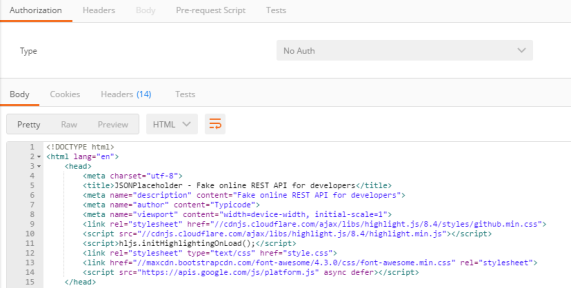
\includegraphics[scale=0.6]{3.png}
\caption{ Postman Aray�z Ekran�}
\end{figure}

1. Authorization : Kimlik do�rulama i�lemi i�in  buradan ona uygun formatta de�erler girilir.

2. Header : Request bilgileriyle birlikte g�nderilecek header de�erleri girilir.

3. Body : Aktif hale gelmesi i�in men�den "POST" se�ilmesi gerekmektedir.  Ve post de�erleri kar�� tarafa.4 farkl� �ekilde g�nderilebilinilir.

a) form-data  b) x-www-form-urlencoded  c) raw d) binary

Raw'� se�ip ve Json format�nda veriler set edilir.
\begin{figure}[H]
\centering
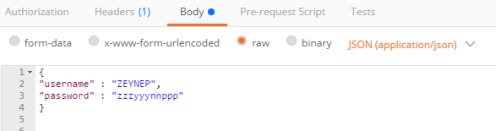
\includegraphics[scale=0.6]{5.png}
\caption{ Postman Veri G�nderme}
\end{figure}

4. Response Body : Body tab�nda d�nen de�erler geliyor ve ��kt�y� 3 farkl� formatta veriyor.

a) Pretty  b)Raw  c)Preview


\begin{figure}[H]
\centering
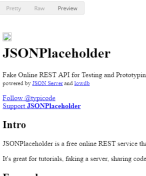
\includegraphics[scale=0.6]{6.png}
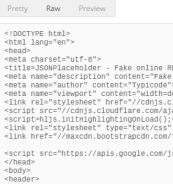
\includegraphics[scale=0.6]{4.png}
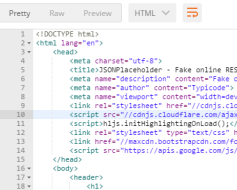
\includegraphics[scale=0.6]{7.png}
\caption{ Postman D�nen Veriler}
\end{figure}
\section{ASP.NET WEB API NED�R?}

\qquad Web Api'ye ge�meden �nce Api nedir ondan bahsedeyim. Api a��l�m� "Application Programming Interface" olan T�rk�e'de uygulama geli�tirme aray�z� anlam�na gelir ve sahip oldu�umuz service veya verileri d�� d�nyaya a��p ba�ka uygulamalar�n-platformlar�n kullan�m�na sunmak i�in belli kurallar �er�evesinde tan�mlamalar yapt���m�z aray�z'd�r.

\qquad Asp .Net Web Api ise farkl� t�rde say�s�z client (browsers, mobile phones, tablets, pc, etc.) taraf�ndan consume edilebilen HTTP protokol� �zerinden haberle�ebilen servisler olu�turmak i�in kullan�lan bir framework �eklinde tan�mlayabiliriz. Asp .net MVC ile routing, controllers, action results, filter, model binders gibi ortak feature'lara sahip olduklar�ndan bir tak�m benzerlikler g�stermektedir ancak MVC Framework'�n bir par�as� de�ildir. Asp .net Web Api Core Asp .Net'in bir par�as�d�r ve MVC veya di�er web application t�rleri ile birlikte kullan�labilir. Ayn� zamanda b�t�n bunlardan ba��ms�z stand-alone Web services application olarakta kullan�labilir.
 
\qquad G�n�m�z d�nyas�nda teknolojinin geli�mesiyle birlikte firmalar art�k web tabanl� uygulamalar �zerinden m��terilerine tam olarak ula�amaz hale geldiler. �nsanlar art�k g�nl�k hayatlar�n�n nerdeyse \%50 sini ak�ll� telefonlar, tablet pc vs ile ge�iriyorlar ve bu cihazlarda insanlar�n hayatlar�n� kolayla�t�racak olan milyonlarca uygulama mevcut. Bunlar�n yan�nda birde IOT ile birlikte gelecek 5 y�lda d�nyada 30 milyara yak�n internete ba�lanabilen cihazlar olaca��ndan bahsediliyor ve buda belki milyonlarca Api geli�tirmesi demek.

\qquad Firmalar veya uygulama geli�tiriciler m��terilere daha kolay ve h�zl� bir �ekilde ula�mada kullanmak i�in servislerini ve sahip olduklar� verilerin bir k�sm�n� browserlar ya da internete ba�lanabilen bu ak�ll� cihazlar taraf�ndan consume edilebilmeleri i�in Api'lar geli�tirmeleri gerekmektedir. ��nk� Api'lar yap�s� gere�i b�t�n programlama dilleri taraf�ndan ortak kabul g�rm�� medya tiplerini (XML-JOSN..etc.) response olarak al�p gerekli parse i�lemlerinden sonra kolayca kullanabilir. 

\qquad Web Api sahip oldu�unuz veri ve servisleri bir�ok farkl� cihazda kullan�ma sunmak i�in expose edebilmenizi sa�layan �ahane bir framework ve dahas� Web Api .Net Framework �zerinde RESTful servisler in�a etmenizi sa�layacak ideal bir open source platform. WCF Rest service'lerinin aksine Web Api HTTP protokol�n�n b�t�n �zelliklerini kullan�r (URIs, request/response headers, caching, versioning, �e�itli content format'lar�) WCF Rest Service'lerinde yap�ld��� gibi farkl� cihazlar i�in extra config ayarlar� vs yapmam�za da gerek bulunmamaktad�r. Request'i yap�l�rken d�nmesi gereken response'un XML mi yoksa JSON format�nda m� olaca��na client'�n se�imine b�rak�lm��t�r.  ��nk� Web Api birden fazla medya format�nda response d�nebilmektedir.

Ba�l�ca Web API �zellikleri
\begin{itemize}
\item Http Get, Post, Put ve Delete metodlar�yla �al��abildi�inden CRUD i�lemelrini destekler,
\item Response'larda HttpStatusCode ve Accept Header parametreleri bulunur,
\item Response'lar kullan�c�n�n istedi�i t�rde MediaTypeFormatter taraf�ndan formatlanabilir,
\item  OData deste�i bulunmaktad�r ve Query yazmas� olduk�a kolayd�r,
\item Bir uygulama i�erisinde veya IIS �zerinde host edilebilir,
\item MVC'nin baz� �zelliklerini ta��r (routing, controllers, action results, filter, model binders)
 
\end{itemize}

\pagebreak
Neden Web Api'� Se�meliyiz ?
\begin{itemize}
\item Bir web service'e ihtiyac�n�z varsa ve soap'a ihtiyac�n�z yoksa en iyi se�enek Web Api dir,
\item Geli�tirme s�rece WCF de oldu�u kadar zahmetli ve s�k�nt�l� de�ildir,
\item 	Http tabanl� oldu�undan Rest-ful servisler geli�tirmek i�in en iyi se�enektir,
\item Exception ve Cache mimarileri olduk�a performansl� ve y�netilebilir dir,
\item Open Source oldu�undan s�rekli olarak geli�tirilip yeni feature'lar eklenmektedir,
\item Microsoft yetkilileri Web Api sunumlar�ndan birinde �una benzer bir �ey s�yledi "Biz daha iyisini yapana kadar en iyisi bu..!" bu demek oluyor ki tam destek[3].
\end{itemize}

\section{G�R�NT� ��LEME NED�R?}
\qquad G�r�nt� i�leme, bir g�r�nt�y� dijital form haline getirmek ve baz� i�lemleri ger�ekle�tirmek i�in geli�tirilmi� bir g�r�nt� elde etmek veya ondan baz� yararl� bilgiler ��karmak i�in kullan�lan bir y�ntemdir. Bu, video �er�evesi veya foto�raf gibi bir girdinin g�r�nt�n�n oldu�u ve ��kt� ile ili�kili g�r�nt� veya karakteristik olabilen bir sinyal tutma t�r�d�r. Genellikle G�r�nt� ��leme sistemi, g�r�nt�leri �nceden tan�mlanm�� sinyal i�leme y�ntemleri uygularken iki boyutlu sinyaller olarak i�ler.
\subsection{�ALI�MA MANTI�I NED�R?}

\qquad G�r�nt� i�leme temel olarak a�a��daki �� ad�m� i�erir.
\begin{enumerate}
\item G�r�nt�n�n optik taray�c�  veya dijital foto�raflarla al�nmas�.
\item Veri s�k��t�rma, g�r�nt� iyile�tirmeye ve uydu foto�raflar� gibi insan g�zleri i�in olmayan lekelenme kal�plar�n� i�eren g�r�nt�y� analiz etme ve kullanma.
\item ��kt�, sonu�lar�n imge analizine dayanan g�r�nt� veya rapor de�i�tirilebilen  son a�amas�d�r.
\end{enumerate}
\subsection{G�R�NT� ��LEMEN�N AMACI NED�R?}

\qquad G�r�nt� i�lemenin amac�n� be�  maddede �zetleyebiliriz:
\begin{enumerate}
\item G�rselle�tirme: g�r�nmeyen nesneleri g�zlemlemek i�in kullan�r�z.
\item G�r�nt� Keskinle�tirme Ve Restorasyon: G�r�nt� netle�tirme ve daha iyi g�r�nt� almak i�in kullan�r�z.
\item  G�r�nt� Al�m�: �lgi �eken g�r�nt�ler i�in kullan�r�z.
\item Desen �l��m�: G�r�nt�deki �e�itli nesneleri tespit etmek i�in kullan�r�z.
\item Resim Tan�ma: G�r�nt�deki �e�itli nesneleri ay�rt etmek i�in kullan�r�z.
\end{enumerate}
\subsection{G�R�NT� ��LEME T�RLER�}

\qquad G�r�nt� i�leme i�in kullan�lan iki y�ntem  Analog G�r�nt� ��leme ve Dijital G�r�nt� ��leme y�ntemidir. Bask� ve foto�raf gibi bas�l� kopyalar i�in analog veya g�rsel g�r�nt� i�leme teknikleri kullan�labilir. G�r�nt� analistleri, bu g�rsel teknikleri kullan�rken yorumlaman�n �e�itli temellerini kullan�l�rlar. G�r�nt� i�leme sadece incelenmesi gereken alanla s�n�rl� de�il analist bilgisi �zerine de yap�labilir. G�rsel tekniklerle g�r�nt� i�leme  alan�ndaki bir di�er �nemli ara� da birlikteliktir. Bu y�zden analistler, ki�isel bilgi ve teminat verilerini bir arada g�r�nt� i�leme i�lemine tabi tutarlar[4].

\qquad Dijital ��leme teknikleri dijital g�r�nt�lerin bilgisayarlarla d�zenlenmesine yard�mc� olur. Uydu platformundan g�r�nt� alg�lay�c�lar�na ait ham veriler eksiklik i�erdi�inden bu kusurlar� a�mak ve bilginin �zg�nl���n� elde etmek i�in, �e�itli i�lem ve a�amalardan ge�mek zorundad�r. Her t�rl� verinin dijital tekni�i kullan�rken ge�mesi gereken �� genel a�ama;
\begin{enumerate}
\item �n ��leme
\item Geli�tirme ve G�r�nt�leme
\item Bilgi ��kar�m�'d�r.
\end{enumerate}
	\subsection{G�R�NT� ��LEME TEKNOLOJ�S�N�N KULLANILDI�I ALANLAR}
\begin{itemize}
\item �r�n Sayma ve Hata Tespiti
\item Uydu G�r�nt�leri �zerinde N�fus Yo�unlu�u, �evre Kirlili�i Ve Benzeri �evresel �artlar�n Tespiti
\item Kalite, Do�ruluk ve Y�zey Analizi
\item Askeri End�stri (Denizalt� Sonic Dalga Taramalar�), Sualt� G�r�nt�leme
\item Robot Kol Y�netimi
\item Eksik, Hatal� Par�a veya �retim Kontrol�
\item Robotik, Trafik, Astronomi, Radar, Gazete Ve Foto�raf End�strisi Uygulamalar�
\item Fizik, Sanat, Biyomedikal Alanlar
\item Uzaktan Alg�lama Uygulamalar�
\item Uydu G�r�nt�leri �zerinde Hava G�zlem ve Tahmin Uygulamalar�
\end{itemize}
\pagebreak
\section{WEB API �LE G�R�NT� ��LEME UYGULAMASI}
\subsection{Y�Z TANIMA NED�R?}
\qquad Bir y�z da�arc��� i�erisinde bir ki�inin y�z�n� tespit edip o ki�iyi bulma i�lemine y�z tan�ma denir. Y�z tan�ma i�lemi �ncelikle y�z�n tespiti ve daha sonra tespit edilen bu y�z�n veritaban�ndaki y�z da�arc���yla �e�itli y�ntemleri (PCA, LDA, EP, ICA vb.) kullanarak bulma i�lemidir.

\qquad Matlab'da ki�i say�s�n� bulabilmek i�in �ncelikle resimdeki y�zleri bulmak gerekmektedir. Bir resim i�inde y�z�n konumunu tespit etmek i�in Matlab'�n i�inde bulunan Viola-Jones algoritmas� kullanarak nesneleri alg�lama i�lemi yapan Cascade nesne dedekt�r�n� kullan�l�r. Cascade nesne dedekt�r� uygulanan resim i�erisinde buldu�u y�zlerin resim �zerindeki x ve y eksenine g�re koordinatlar�n� vermektedir. Temel olarak dedekt�r y�z alg�lamak �zere yap�land�r�lm��, fakat di�er nesne t�rleri i�in yap�land�r�labilir.

\begin{figure}[H]
\centering
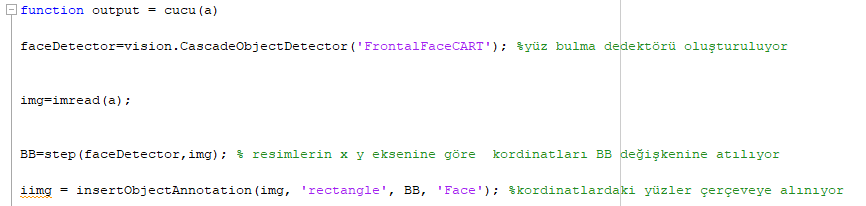
\includegraphics[scale=0.6]{1.png}

\caption{ Y�z Bulma Kodu}
\end{figure}
\pagebreak
\qquad Bulunan y�zleri �er�eveye ald�ktan sonra klas�re kaydedilir. Burada klas�re y�zleri yerle�tirmek i�in isim verilir. Verilen ismi counter ad�nda bir saya� olu�turarak say�sal olarak tan�mland�. For d�ng�s� i�erinde tekrardan ksayisi ad�nda saya� olu�turarak ki�i say�s� bulunur.
\begin{figure}[H]
\centering
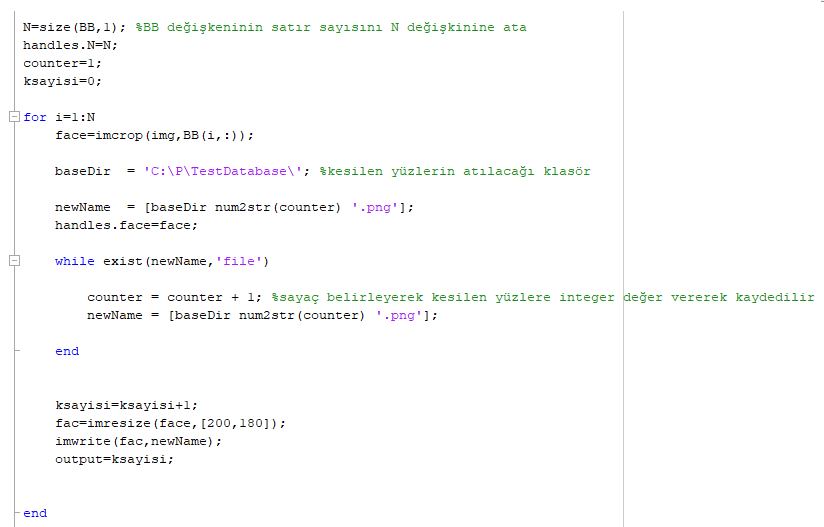
\includegraphics[scale=0.7]{2.png}

\caption{Bulunan Y�zleri Klas�re Atma ve Ki�i Say�s�n� Bulma Kodu}
\end{figure}

\subsection{MATLAB'DA DLL OLU�TURMA}
\qquad Matlab'da dll olu�turmak i�in Command Window penceresine 'deploytool' yaz�l�r. Daha sonra a��lan Compiler penceresinde Library Compiler se�ilir.
\begin{figure}[H]
\centering
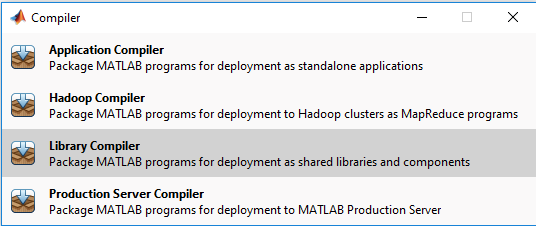
\includegraphics[scale=0.8]{8.png}

\caption{Compiler Penceresi}
\end{figure}

\qquad Dll'i Visual Studio'da �al��t�rmak i�in .Net Assembly'i se�ilir. Daha sonra  .m uzant�l� Matlab dosyas� eklenir. Package'ye t�klayarak dll'in olu�turulaca�� klas�r se�ilerek i�lem tamamlanm�� olur.

\begin{figure}[H]
\centering
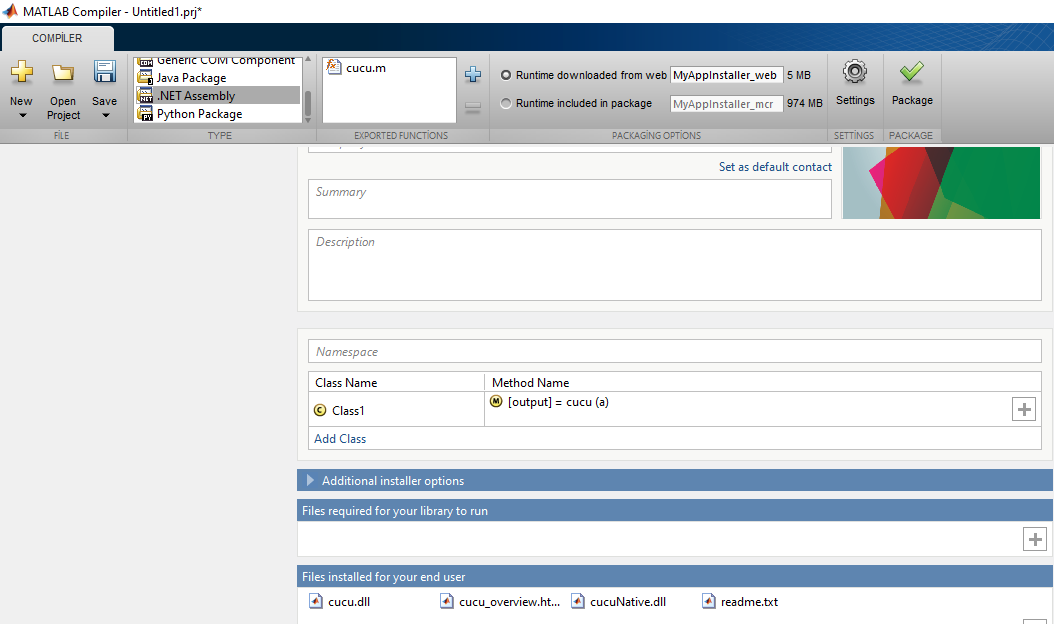
\includegraphics[scale=0.5]{9.png}

\caption{Dll Olu�turma}
\end{figure}
\pagebreak
\subsection{VISUAL STUDIO'DA FILE UPLOAD}

 
\qquad Bu uygulamay� ger�ekle�tirmek i�in ilk olarak dosyadan resim belirlemek gerekir. �ncelikle projede HomeController i�ine Index ad�nda bir action olu�turulur. Index'e sa� t�klay�p View olu�turularak projenin dosya y�kleme i�lemi ger�ekle�tirilir. Bu i�lem i�in metodunu post, enctype'� multipart/form-data olarak tan�mlan�r.

\qquad Div olu�turduktan sonra i�erisine bir adet input > file ve bir adet button > submit kontrolleri yerle�tirilir. �nput > file kontrol�n�n name �zelli�i Image olarak ayarland�. Bu tan�m controller i�erisinde kullan�l�r.

\begin{figure}[H]
\centering
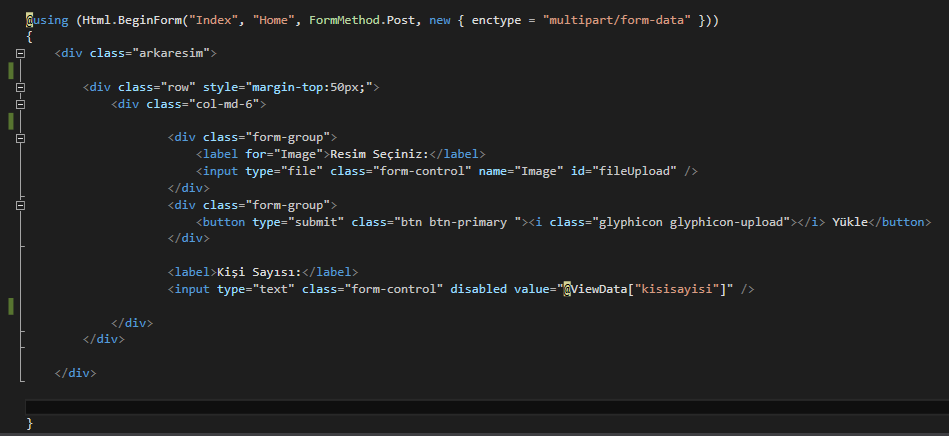
\includegraphics[scale=0.6]{11.png}

\caption{Index Sayfas� Kodlar�}
\end{figure}

\begin{figure}[H]
\centering
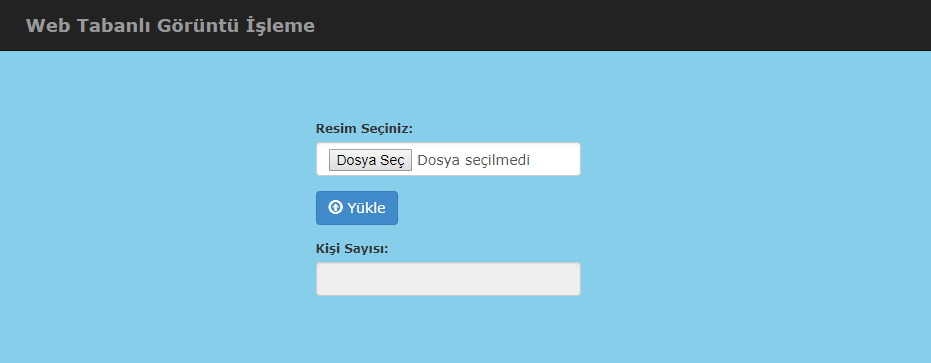
\includegraphics[scale=0.6]{10.png}

\caption{Index Sayfas� }
\end{figure}
\pagebreak
\subsection{VISUAL STUDIO'DA MATLAB FONKS�YONLARINI �ALI�TIRMA}
\qquad HomeController'da yaz�lan dll'li �a��r�l�r. Resmi belirledikten sonra y�kle butonuna t�klayarak olu�turulan dll'e g�nderilir.
\begin{figure}[H]
\centering
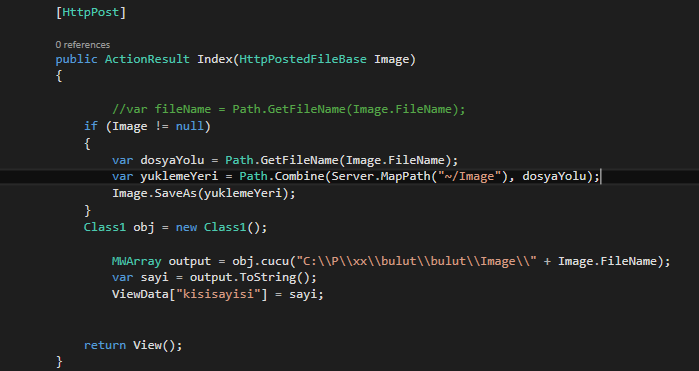
\includegraphics[scale=0.7]{12.png}

\caption{Dll'den Resimdeki Ki�i Say�s�n� �ekme }
\end{figure}

\begin{figure}[H]
\centering
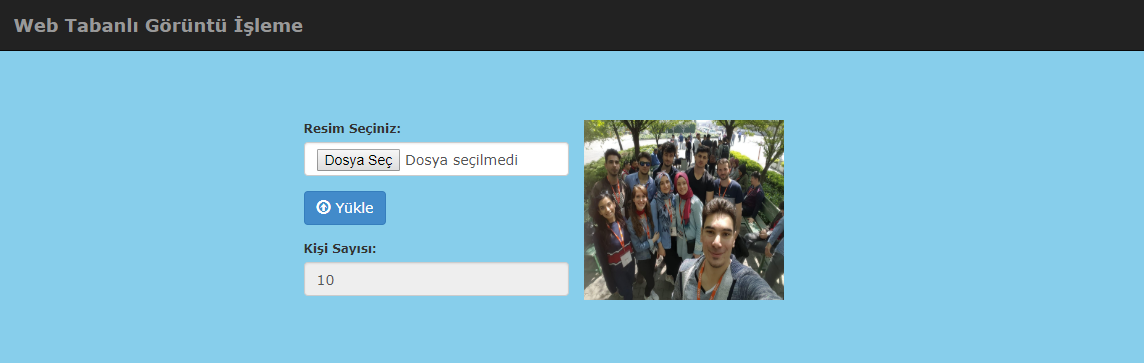
\includegraphics[scale=0.4]{13.png}

\caption{Index Sayfas�n�n Son Hali }
\end{figure}
\pagebreak
\subsection{POSTMAN'DE WEB API TEST�}
\qquad Web Api'de ilk yap�lmas� gereken olu�turulacak Controller'� Web Api2 format�nda se�mektir. Daha sonra burada  class olu�turularak sunucuda depolanacak resmin yolu saklan�r.
Matlab dll'line g�nderilecek resmin yolu yaz�l�r ve sonucu d�nd�r�l�r.
\begin{figure}[H]
\centering
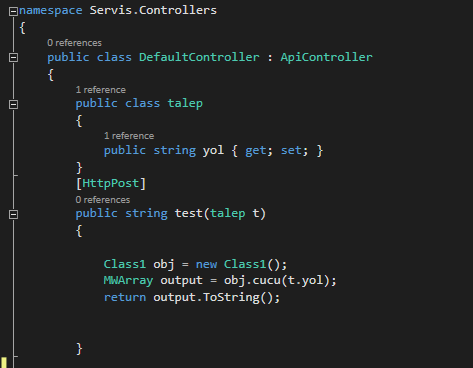
\includegraphics[scale=0.6]{15.png}

\caption{Web Api Kodlar� }
\end{figure}
\begin{figure}[H]
\centering
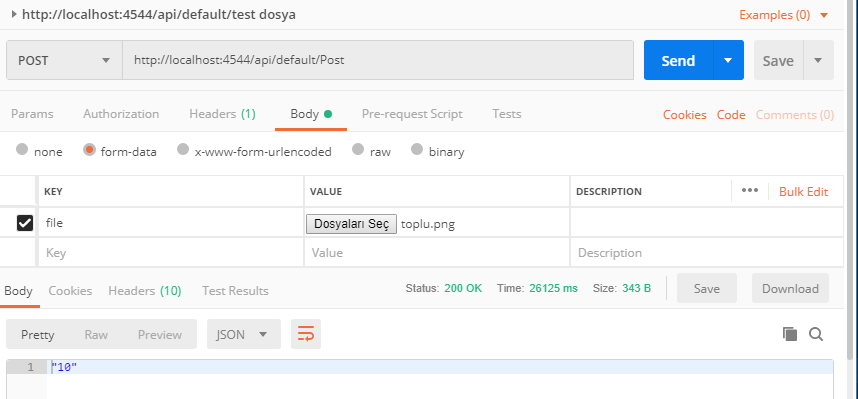
\includegraphics[scale=0.6]{14.png}

\caption{Postman'de Test }
\end{figure}
%\section{ADI}

\section{SONU�LAR VE �NER�LER}
\qquad Hepimiz bilgisayar teknolojisinde ve g�r�nt� i�lemede h�zl� geli�me ile ate�lenen devrimin ortas�nday�z. Bilinen inanca kar��n, bilgisayarlar g�r�nt� i�leme ve analiz ile ilgili hesaplamalarda insanlarla e�le�emez. Ancak modern bilgisayar�n artan geli�mi�li�i ve g�c� ile hesaplama Von Neumann ard���k mimarinin �tesine ge�ecek ve optik y�r�tmeyi de d���necektir. Paralel da��t�lm�� bilgi i�lem paradigmalar�n�n, g�r�nt� i�leme sonu�lar� i�in tepkileri geli�tirmesi beklenmektedir. 


\qquad Ayr�yeten yeni bir teknoloji olan Bulut bili�im de g�zleri �zerine �ekmi�tir.
 
 Bulut bili�im, ���nc� parti yaz�l�mlar taraf�ndan desteklenen ortak bir hesaplama, depolama, a� ve uygulama yaz�l�m�
platformudur. Bulut teknolojisi, kullan�c�lar�n b�y�k miktarlardaki verileri i�lemesi ve hesaplamalar� yapabilmesi i�in
soyutlanm�� ve sanalla�t�r�lm�� bili�im kaynaklar�n� kullanmas�n� sa�lar. Bulut bili�imin bir di�er �nemli avantaj� da, uzak
mesafedeki ara�t�rmac�lar�n verileri payla�mak yoluyla ortak �al��ma yapabilmesidir. Bu �al��mada, bulut bili�im
platformu �zerinde �al��an web tabanl� bir g�r�nt� i�leme uygulamas� ger�ekle�tirilmek istenmi�tir. Ancak  kar��la��lan hatalar neticesinde projenin bulut bili�im k�sm� ger�ekle�tirilememi�tir.



\section{EKLER}

\subsection{MATLAB KODLARI}
\qquad 

 Matlab'da bir resimdeki ki�i say�s�n� bulabilmek i�in  ilk olarak Casced nesne ded�kt�r� ile y�zler bulundu. Daha sonra  bulunan y�zler TestDatabase adl� klas�re kydedilir. For d�ng�s� i�erine saya� konularak kaydedilen resim say�s� bulunur. Bu da resimdeki ki�i say�s�n� verir.

\lstinputlisting[]{cucu.m}
\subsection{VISUAL STUDIO KODLARI}
\qquad Visual Studio i�in ilk olarak dosyadan resim belirlemek gerekir. �ncelikle projede HomeController i�ine Index ad�nda bir action olu�turulur. Index'e sa� t�klay�p View olu�turularak projenin dosya y�kleme i�lemi ger�ekle�tirilir. Bu i�lem i�in metodunu post, enctype'� multipart/form-data olarak tan�mlan�r.

\qquad Div olu�turduktan sonra i�erisine bir adet input > file ve bir adet button > submit kontrolleri yerle�tirilir. �nput > file kontrol�n�n name �zelli�i Image olarak ayarland�. Bu tan�m controller i�erisinde kullan�l�r.

\subsubsection{HomeController.cs}
\lstinputlisting[]{HomeController.cs}\subsubsection{Index.cshtml}
 @ \{
 
    ViewBag.Title = "Index";
    
    string dosyayolu = TempData["dosyayolu"] as string;
    
\}
    <style>
 
      body \{
      
            background-color:skyblue;
            
            background-repeat: no-repeat;
            
            background-attachment: fixed;

            font-family: Verdana, monospace, sans-serif;
            
            font-size: 12px;
            
            font-weight: bold;
            
            text-align: justify;
            
            min-height: 800px;
            
        \}
     div.arkaresim \{
     
          width: 600px;
          
          height: 300px;
          
          padding: 20px;
          
          background-color: skyblue;
          
          position: relative;
          
          margin: auto;
          
    \}

    </style>
   
@using (Html.BeginForm("Index", "Home", FormMethod.Post, 

new \{ enctype = "multipart/form-data" \}))

\{
    <div class="arkaresim">
        
        <div class="row" style="margin-top:50px;">
        
            <div class="col-md-6">
               
                    <div class="form-group">
                    
<label for="Image">Resim Se�iniz:</label>

<input type="file" class="form-control" name="Imagee" id="fileUpload" />

                    </div>
                    
                    <div class="form-group">
                    
                        <button type="submit" class="btn btn-primary ">
                        
						<i class="glyphicon glyphicon-upload"></i>
						
						 Y�kle</button>
						 
                    </div>

                    <label>Ki�i Say�s�:</label>
                    
                    <input type="text" class="form-control" 
                    
                    disabled value="@ViewData["kisisayisi"]" />
                    
</div>          
<div class="result">
            
<img src="~/Image/@dosyayolu" width="200" height="180" alt="image" />

            </div>
            
        </div>
        
    </div>
    
\}


\subsubsection{DefaultController.cs}
\lstinputlisting[]{DefaultController.cs}
\renewcommand{\refname}{KAYNAKLAR}
\addcontentsline{toc}{section}{KAYNAKLAR}
\begin{thebibliography}{99}%kaynak ortam� olu�turmak i�in
%%%%Kaynak Web sayfas�ndan al�nm�� ise%%%%%%%%%%%%%%%%%
\bibitem{k:1} CTAN,\url{http://www.wikizeroo.net/index.php?
q=aHR0cHM6Ly90ci53aWtpcGVkaWEub3JnL3dpa

2kvTUFUTEFC} 


\bibitem{k:2}  CTAN,\url{http://www.wikizeroo.net/index.php?q=aHR0cHM6Ly90ci53aWtpcGVkaWEub3JnL
3dpa2kvTWljcm9zb2Z0X1Zpc3VhbF9TdHVkaW8} 

\bibitem{k:3} \url{http://www.canertosuner.com/post/Web-Api-Nedir}
\bibitem{k:4} \url{https://www.mustafasaridal.com/goruntu-isleme/goruntu-isleme-teknolojisi-image-processing-nedir/}

\bibitem{k:5} \url{https://cevirsozluk.com//}
\end{thebibliography}
\centerline{\textbf{�ZGE�M��}}
\addcontentsline{toc}{section}{�ZGE�M��}
\begin{table}[H]
{
\renewcommand{\arraystretch}{1.5}
\begin{tabular}{l@{\bf :}l}
\multicolumn{2}{l}{\underline{\bf K���SEL B�LG�LER}}\cr
\textbf{Ad� Soyad�}&   Zeynep KOTAN  \cr
\textbf{Uyru�u}&\; T.C. \cr
\textbf{Do�um Yeri ve Tarihi}&\;  A�kale  /04.08.1997 \cr
\textbf{Adres}&\;   G�ne�li 15Temmuz mah. 1402.sokak no:19/2 Ba�c�lar/�ST    \cr
\multicolumn{1}{l}{}&      \cr
\textbf{Telefon}&\; 539 565 2406    \cr
\textbf{e-mail}&\;  zeynepkotan1@gmail.com \cr
\multicolumn{1}{l}{}&\cr
\multicolumn{2}{l}{\underline{\bf E��T�M DURUMU}}\cr
\textbf{Lisans ��renimi}&\; B�E� Bilgisayar M�hendisli�i B�l�m�\cr
\textbf{Bitirme Y�l�}&\;    \cr
\textbf{Lise}& \; Ahi Evren Anadolu �HL   \cr
\multicolumn{1}{l}{}&\cr
\multicolumn{2}{l}{\underline{\bf �� DENEY�MLER�}}\cr
\textbf{Y�l}&\;     \cr
\textbf{Kurum}& \;    \cr
\textbf{Stajlar}&\;   Staj1  \cr
\multicolumn{1}{l}{}&\cr
\multicolumn{2}{l}{\underline{\bf �LG� ALANLARI:}}\cr
\multicolumn{1}{l}{}&\cr
\multicolumn{2}{l}{\underline{\bf YABANCI D�LLER:} �ngilizce:Orta Arap�a:Ba�lang��}\cr
\multicolumn{1}{l}{}&\cr
\multicolumn{2}{l}{\underline{\bf BEL�RTMEK �STED���N�Z D��ER �ZELL�KLER:}}
\end{tabular}}
\end{table}
\shorthandon{=}
\end{document}
%%%%%%%%%%%%%%%%%%%%%%%%%%%B�TT�%%%%%%%%%%%%%%%%%%%%%%%%%%%%%%%%%%%%%%%%%%%%%
